% Options for packages loaded elsewhere
\PassOptionsToPackage{unicode}{hyperref}
\PassOptionsToPackage{hyphens}{url}
\PassOptionsToPackage{dvipsnames,svgnames,x11names}{xcolor}
%
\documentclass[
  letterpaper,
  DIV=11,
  numbers=noendperiod]{scrartcl}

\usepackage{amsmath,amssymb}
\usepackage{iftex}
\ifPDFTeX
  \usepackage[T1]{fontenc}
  \usepackage[utf8]{inputenc}
  \usepackage{textcomp} % provide euro and other symbols
\else % if luatex or xetex
  \usepackage{unicode-math}
  \defaultfontfeatures{Scale=MatchLowercase}
  \defaultfontfeatures[\rmfamily]{Ligatures=TeX,Scale=1}
\fi
\usepackage{lmodern}
\ifPDFTeX\else  
    % xetex/luatex font selection
\fi
% Use upquote if available, for straight quotes in verbatim environments
\IfFileExists{upquote.sty}{\usepackage{upquote}}{}
\IfFileExists{microtype.sty}{% use microtype if available
  \usepackage[]{microtype}
  \UseMicrotypeSet[protrusion]{basicmath} % disable protrusion for tt fonts
}{}
\makeatletter
\@ifundefined{KOMAClassName}{% if non-KOMA class
  \IfFileExists{parskip.sty}{%
    \usepackage{parskip}
  }{% else
    \setlength{\parindent}{0pt}
    \setlength{\parskip}{6pt plus 2pt minus 1pt}}
}{% if KOMA class
  \KOMAoptions{parskip=half}}
\makeatother
\usepackage{xcolor}
\setlength{\emergencystretch}{3em} % prevent overfull lines
\setcounter{secnumdepth}{-\maxdimen} % remove section numbering
% Make \paragraph and \subparagraph free-standing
\makeatletter
\ifx\paragraph\undefined\else
  \let\oldparagraph\paragraph
  \renewcommand{\paragraph}{
    \@ifstar
      \xxxParagraphStar
      \xxxParagraphNoStar
  }
  \newcommand{\xxxParagraphStar}[1]{\oldparagraph*{#1}\mbox{}}
  \newcommand{\xxxParagraphNoStar}[1]{\oldparagraph{#1}\mbox{}}
\fi
\ifx\subparagraph\undefined\else
  \let\oldsubparagraph\subparagraph
  \renewcommand{\subparagraph}{
    \@ifstar
      \xxxSubParagraphStar
      \xxxSubParagraphNoStar
  }
  \newcommand{\xxxSubParagraphStar}[1]{\oldsubparagraph*{#1}\mbox{}}
  \newcommand{\xxxSubParagraphNoStar}[1]{\oldsubparagraph{#1}\mbox{}}
\fi
\makeatother

\usepackage{color}
\usepackage{fancyvrb}
\newcommand{\VerbBar}{|}
\newcommand{\VERB}{\Verb[commandchars=\\\{\}]}
\DefineVerbatimEnvironment{Highlighting}{Verbatim}{commandchars=\\\{\}}
% Add ',fontsize=\small' for more characters per line
\usepackage{framed}
\definecolor{shadecolor}{RGB}{241,243,245}
\newenvironment{Shaded}{\begin{snugshade}}{\end{snugshade}}
\newcommand{\AlertTok}[1]{\textcolor[rgb]{0.68,0.00,0.00}{#1}}
\newcommand{\AnnotationTok}[1]{\textcolor[rgb]{0.37,0.37,0.37}{#1}}
\newcommand{\AttributeTok}[1]{\textcolor[rgb]{0.40,0.45,0.13}{#1}}
\newcommand{\BaseNTok}[1]{\textcolor[rgb]{0.68,0.00,0.00}{#1}}
\newcommand{\BuiltInTok}[1]{\textcolor[rgb]{0.00,0.23,0.31}{#1}}
\newcommand{\CharTok}[1]{\textcolor[rgb]{0.13,0.47,0.30}{#1}}
\newcommand{\CommentTok}[1]{\textcolor[rgb]{0.37,0.37,0.37}{#1}}
\newcommand{\CommentVarTok}[1]{\textcolor[rgb]{0.37,0.37,0.37}{\textit{#1}}}
\newcommand{\ConstantTok}[1]{\textcolor[rgb]{0.56,0.35,0.01}{#1}}
\newcommand{\ControlFlowTok}[1]{\textcolor[rgb]{0.00,0.23,0.31}{\textbf{#1}}}
\newcommand{\DataTypeTok}[1]{\textcolor[rgb]{0.68,0.00,0.00}{#1}}
\newcommand{\DecValTok}[1]{\textcolor[rgb]{0.68,0.00,0.00}{#1}}
\newcommand{\DocumentationTok}[1]{\textcolor[rgb]{0.37,0.37,0.37}{\textit{#1}}}
\newcommand{\ErrorTok}[1]{\textcolor[rgb]{0.68,0.00,0.00}{#1}}
\newcommand{\ExtensionTok}[1]{\textcolor[rgb]{0.00,0.23,0.31}{#1}}
\newcommand{\FloatTok}[1]{\textcolor[rgb]{0.68,0.00,0.00}{#1}}
\newcommand{\FunctionTok}[1]{\textcolor[rgb]{0.28,0.35,0.67}{#1}}
\newcommand{\ImportTok}[1]{\textcolor[rgb]{0.00,0.46,0.62}{#1}}
\newcommand{\InformationTok}[1]{\textcolor[rgb]{0.37,0.37,0.37}{#1}}
\newcommand{\KeywordTok}[1]{\textcolor[rgb]{0.00,0.23,0.31}{\textbf{#1}}}
\newcommand{\NormalTok}[1]{\textcolor[rgb]{0.00,0.23,0.31}{#1}}
\newcommand{\OperatorTok}[1]{\textcolor[rgb]{0.37,0.37,0.37}{#1}}
\newcommand{\OtherTok}[1]{\textcolor[rgb]{0.00,0.23,0.31}{#1}}
\newcommand{\PreprocessorTok}[1]{\textcolor[rgb]{0.68,0.00,0.00}{#1}}
\newcommand{\RegionMarkerTok}[1]{\textcolor[rgb]{0.00,0.23,0.31}{#1}}
\newcommand{\SpecialCharTok}[1]{\textcolor[rgb]{0.37,0.37,0.37}{#1}}
\newcommand{\SpecialStringTok}[1]{\textcolor[rgb]{0.13,0.47,0.30}{#1}}
\newcommand{\StringTok}[1]{\textcolor[rgb]{0.13,0.47,0.30}{#1}}
\newcommand{\VariableTok}[1]{\textcolor[rgb]{0.07,0.07,0.07}{#1}}
\newcommand{\VerbatimStringTok}[1]{\textcolor[rgb]{0.13,0.47,0.30}{#1}}
\newcommand{\WarningTok}[1]{\textcolor[rgb]{0.37,0.37,0.37}{\textit{#1}}}

\providecommand{\tightlist}{%
  \setlength{\itemsep}{0pt}\setlength{\parskip}{0pt}}\usepackage{longtable,booktabs,array}
\usepackage{calc} % for calculating minipage widths
% Correct order of tables after \paragraph or \subparagraph
\usepackage{etoolbox}
\makeatletter
\patchcmd\longtable{\par}{\if@noskipsec\mbox{}\fi\par}{}{}
\makeatother
% Allow footnotes in longtable head/foot
\IfFileExists{footnotehyper.sty}{\usepackage{footnotehyper}}{\usepackage{footnote}}
\makesavenoteenv{longtable}
\usepackage{graphicx}
\makeatletter
\def\maxwidth{\ifdim\Gin@nat@width>\linewidth\linewidth\else\Gin@nat@width\fi}
\def\maxheight{\ifdim\Gin@nat@height>\textheight\textheight\else\Gin@nat@height\fi}
\makeatother
% Scale images if necessary, so that they will not overflow the page
% margins by default, and it is still possible to overwrite the defaults
% using explicit options in \includegraphics[width, height, ...]{}
\setkeys{Gin}{width=\maxwidth,height=\maxheight,keepaspectratio}
% Set default figure placement to htbp
\makeatletter
\def\fps@figure{htbp}
\makeatother

\KOMAoption{captions}{tableheading}
\makeatletter
\@ifpackageloaded{caption}{}{\usepackage{caption}}
\AtBeginDocument{%
\ifdefined\contentsname
  \renewcommand*\contentsname{Table of contents}
\else
  \newcommand\contentsname{Table of contents}
\fi
\ifdefined\listfigurename
  \renewcommand*\listfigurename{List of Figures}
\else
  \newcommand\listfigurename{List of Figures}
\fi
\ifdefined\listtablename
  \renewcommand*\listtablename{List of Tables}
\else
  \newcommand\listtablename{List of Tables}
\fi
\ifdefined\figurename
  \renewcommand*\figurename{Figure}
\else
  \newcommand\figurename{Figure}
\fi
\ifdefined\tablename
  \renewcommand*\tablename{Table}
\else
  \newcommand\tablename{Table}
\fi
}
\@ifpackageloaded{float}{}{\usepackage{float}}
\floatstyle{ruled}
\@ifundefined{c@chapter}{\newfloat{codelisting}{h}{lop}}{\newfloat{codelisting}{h}{lop}[chapter]}
\floatname{codelisting}{Listing}
\newcommand*\listoflistings{\listof{codelisting}{List of Listings}}
\makeatother
\makeatletter
\makeatother
\makeatletter
\@ifpackageloaded{caption}{}{\usepackage{caption}}
\@ifpackageloaded{subcaption}{}{\usepackage{subcaption}}
\makeatother

\ifLuaTeX
  \usepackage{selnolig}  % disable illegal ligatures
\fi
\usepackage{bookmark}

\IfFileExists{xurl.sty}{\usepackage{xurl}}{} % add URL line breaks if available
\urlstyle{same} % disable monospaced font for URLs
\hypersetup{
  pdftitle={Beta-Regression Code for Using Tree-Based Models to Identify Factors Contributing to Trait Negative Affect in Adults with and without Major Depression Manuscript},
  pdfauthor={Catalina Canizares},
  colorlinks=true,
  linkcolor={blue},
  filecolor={Maroon},
  citecolor={Blue},
  urlcolor={Blue},
  pdfcreator={LaTeX via pandoc}}


\title{Beta-Regression Code for Using Tree-Based Models to Identify
Factors Contributing to Trait Negative Affect in Adults with and without
Major Depression Manuscript}
\author{Catalina Canizares}
\date{2023-04-28}

\begin{document}
\maketitle


\section{Loading the data}\label{loading-the-data}

\begin{Shaded}
\begin{Highlighting}[]
\NormalTok{affectivity\_data\_df }\OtherTok{\textless{}{-}}\FunctionTok{read\_excel}\NormalTok{(}\StringTok{"data/Psico\_New.xlsx"}\NormalTok{)}
\end{Highlighting}
\end{Shaded}

\section{Wrangle data}\label{wrangle-data}

\begin{Shaded}
\begin{Highlighting}[]
\NormalTok{rename\_binary }\OtherTok{\textless{}{-}} \ControlFlowTok{function}\NormalTok{(x) \{}
  \FunctionTok{return}\NormalTok{(}
    \FunctionTok{case\_when}\NormalTok{(}
\NormalTok{      x }\SpecialCharTok{==} \DecValTok{1} \SpecialCharTok{\textasciitilde{}} \StringTok{" Yes"}\NormalTok{,}
\NormalTok{      x }\SpecialCharTok{==} \DecValTok{0} \SpecialCharTok{\textasciitilde{}} \StringTok{"No"}
\NormalTok{    )}
\NormalTok{  )}
\NormalTok{\}}

\NormalTok{demographics\_df }\OtherTok{\textless{}{-}}
\NormalTok{  affectivity\_data\_df  }\SpecialCharTok{\%\textgreater{}\%}
  \FunctionTok{select}\NormalTok{(}
    \AttributeTok{Age =}\NormalTok{ EDAD,}
    \StringTok{\textasciigrave{}}\AttributeTok{Disconnection and Rejection}\StringTok{\textasciigrave{}} \OtherTok{=}\NormalTok{ DYRYSQ, }
    \StringTok{\textasciigrave{}}\AttributeTok{Impaired Autonomy}\StringTok{\textasciigrave{}} \OtherTok{=}\NormalTok{ PADYSQ, }
    \StringTok{\textasciigrave{}}\AttributeTok{Impaired Limits}\StringTok{\textasciigrave{}} \OtherTok{=}\NormalTok{LIYSQ, }
    \StringTok{\textasciigrave{}}\AttributeTok{Other{-}Directedness}\StringTok{\textasciigrave{}} \OtherTok{=}\NormalTok{ THOYSQ, }
    \StringTok{\textasciigrave{}}\AttributeTok{Over{-}Vigilance/Inhibition}\StringTok{\textasciigrave{}} \OtherTok{=}\NormalTok{ SEIYSQ,}
    \StringTok{\textasciigrave{}}\AttributeTok{IDER Score}\StringTok{\textasciigrave{}} \OtherTok{=}\NormalTok{ IDERR\_total, }
    \StringTok{\textasciigrave{}}\AttributeTok{Number of Stressful Events}\StringTok{\textasciigrave{}} \OtherTok{=}\NormalTok{ ESVfrec, }
    \AttributeTok{Sex =}\NormalTok{ SEXO,}
    \StringTok{\textasciigrave{}}\AttributeTok{Negative Attribution}\StringTok{\textasciigrave{}} \OtherTok{=}\NormalTok{ dummyPosNeg, }
    \StringTok{\textasciigrave{}}\AttributeTok{Unexpected Attribution}\StringTok{\textasciigrave{}} \OtherTok{=}\NormalTok{ dummyEsInes, }
    \StringTok{\textasciigrave{}}\AttributeTok{Out of Control Attribution}\StringTok{\textasciigrave{}}  \OtherTok{=}\NormalTok{ dummyConNocon,}
    \StringTok{\textasciigrave{}}\AttributeTok{Childhood Adversity}\StringTok{\textasciigrave{}} \OtherTok{=}\NormalTok{ ABUSOINFANCIA, }
    \StringTok{\textasciigrave{}}\AttributeTok{Physical Excercise}\StringTok{\textasciigrave{}} \OtherTok{=}\NormalTok{ deporte, }
    \StringTok{\textasciigrave{}}\AttributeTok{Smoking Cigarettes}\StringTok{\textasciigrave{}} \OtherTok{=}\NormalTok{ fuma, }
    \StringTok{\textasciigrave{}}\AttributeTok{Alcohol Use}\StringTok{\textasciigrave{}} \OtherTok{=}\NormalTok{ Alcohol, }
    \StringTok{\textasciigrave{}}\AttributeTok{Psychoactive Substance Use}\StringTok{\textasciigrave{}} \OtherTok{=}\NormalTok{ psicoactiva}
\NormalTok{    ) }\SpecialCharTok{\%\textgreater{}\%}
  \FunctionTok{mutate}\NormalTok{(}\FunctionTok{across}\NormalTok{(Sex}\SpecialCharTok{:}\StringTok{\textasciigrave{}}\AttributeTok{Psychoactive Substance Use}\StringTok{\textasciigrave{}}\NormalTok{, factor)) }\SpecialCharTok{\%\textgreater{}\%} 
  \FunctionTok{mutate}\NormalTok{(}
    \AttributeTok{Sex =} \FunctionTok{case\_when}\NormalTok{(}
\NormalTok{      Sex }\SpecialCharTok{==} \DecValTok{1} \SpecialCharTok{\textasciitilde{}} \StringTok{"Female"}\NormalTok{,}
\NormalTok{      Sex }\SpecialCharTok{==} \DecValTok{0} \SpecialCharTok{\textasciitilde{}} \StringTok{"Male"}
\NormalTok{    )}
\NormalTok{  ) }\SpecialCharTok{\%\textgreater{}\%}
  \FunctionTok{mutate\_at}\NormalTok{(}
    \FunctionTok{vars}\NormalTok{(}
      \StringTok{\textasciigrave{}}\AttributeTok{Negative Attribution}\StringTok{\textasciigrave{}}\SpecialCharTok{:}\StringTok{\textasciigrave{}}\AttributeTok{Psychoactive Substance Use}\StringTok{\textasciigrave{}}\NormalTok{),}
      \SpecialCharTok{\textasciitilde{}} \FunctionTok{rename\_binary}\NormalTok{(.)) }
\end{Highlighting}
\end{Shaded}

\subsection{Beta Regression}\label{beta-regression}

\begin{Shaded}
\begin{Highlighting}[]
\CommentTok{\# I have to transform the outcome to be from 0 to 1 given that it is a score that only goes from 10 to 40, it is bounded. This function was created by Dr. Gabriel Odom. Please find the documentation in script named liker\_squeezer\_202303314}

\NormalTok{Squeeze }\OtherTok{\textless{}{-}} \ControlFlowTok{function}\NormalTok{(xBdd, lower, upper, }\AttributeTok{squeeze =} \FloatTok{0.5}\NormalTok{) \{}
\NormalTok{    N }\OtherTok{\textless{}{-}} \FunctionTok{length}\NormalTok{(xBdd)}
\NormalTok{    x1 }\OtherTok{\textless{}{-}}\NormalTok{ (xBdd }\SpecialCharTok{{-}}\NormalTok{ lower) }\SpecialCharTok{/}\NormalTok{ (upper }\SpecialCharTok{{-}}\NormalTok{ lower)}
\NormalTok{    x2 }\OtherTok{\textless{}{-}}\NormalTok{ (x1 }\SpecialCharTok{*}\NormalTok{ (N }\SpecialCharTok{{-}} \DecValTok{1}\NormalTok{) }\SpecialCharTok{+}\NormalTok{ squeeze) }\SpecialCharTok{/}\NormalTok{ N}
\NormalTok{    x2}
    
\NormalTok{\}}

\CommentTok{\# Transforming the variable}
\NormalTok{affectivity\_df }\OtherTok{\textless{}{-}}\NormalTok{ demographics\_df }\SpecialCharTok{\%\textgreater{}\%} 
  \FunctionTok{mutate}\NormalTok{(}\AttributeTok{IDER =} \FunctionTok{Squeeze}\NormalTok{(}
    \AttributeTok{xBdd =}\NormalTok{ demographics\_df}\SpecialCharTok{$}\StringTok{\textasciigrave{}}\AttributeTok{IDER Score}\StringTok{\textasciigrave{}}\NormalTok{,}
      \AttributeTok{lower =} \DecValTok{10}\NormalTok{L, }\AttributeTok{upper =} \DecValTok{40}\NormalTok{L}
\NormalTok{    )}
\NormalTok{  ) }\SpecialCharTok{\%\textgreater{}\%} 
  \FunctionTok{select}\NormalTok{(}\SpecialCharTok{{-}}\StringTok{\textasciigrave{}}\AttributeTok{IDER Score}\StringTok{\textasciigrave{}}\NormalTok{)}
\end{Highlighting}
\end{Shaded}

\begin{Shaded}
\begin{Highlighting}[]
\NormalTok{beta\_fit }\OtherTok{\textless{}{-}} \FunctionTok{betareg}\NormalTok{(IDER }\SpecialCharTok{\textasciitilde{}}\NormalTok{ ., }\AttributeTok{data =}\NormalTok{ affectivity\_df)}
\NormalTok{summary\_beta }\OtherTok{\textless{}{-}} \FunctionTok{summary}\NormalTok{(beta\_fit)}
\NormalTok{conf\_ints }\OtherTok{\textless{}{-}} \FunctionTok{confint}\NormalTok{(beta\_fit, }\AttributeTok{level =} \FloatTok{0.95}\NormalTok{)}

\NormalTok{summary\_beta}
\end{Highlighting}
\end{Shaded}

\begin{verbatim}

Call:
betareg(formula = IDER ~ ., data = affectivity_df)

Quantile residuals:
    Min      1Q  Median      3Q     Max 
-3.4633 -0.6360 -0.0989  0.5649  6.2435 

Coefficients (mean model with logit link):
                                 Estimate Std. Error z value Pr(>|z|)    
(Intercept)                    -1.8240348  0.3952193  -4.615 3.93e-06 ***
Age                            -0.0103167  0.0040793  -2.529 0.011437 *  
`Disconnection and Rejection`   0.0636254  0.0164024   3.879 0.000105 ***
`Impaired Autonomy`             0.0798309  0.0163999   4.868 1.13e-06 ***
`Impaired Limits`               0.0192334  0.0125646   1.531 0.125827    
`Other-Directedness`            0.0009408  0.0123753   0.076 0.939404    
`Over-Vigilance/Inhibition`     0.0006187  0.0131395   0.047 0.962443    
`Number of Stressful Events`   -0.0015294  0.0056149  -0.272 0.785324    
SexMale                         0.0718595  0.1009377   0.712 0.476515    
`Negative Attribution`No       -0.4110667  0.1167578  -3.521 0.000430 ***
`Unexpected Attribution`No      0.0432397  0.1031468   0.419 0.675066    
`Out of Control Attribution`No -0.2971213  0.1176300  -2.526 0.011540 *  
`Childhood Adversity`No        -0.3363619  0.0936297  -3.592 0.000328 ***
`Physical Excercise`No          0.0268285  0.0931060   0.288 0.773232    
`Smoking Cigarettes`No         -0.2852899  0.1168429  -2.442 0.014620 *  
`Alcohol Use`No                -0.0487717  0.1295649  -0.376 0.706599    
`Psychoactive Substance Use`No  0.3603303  0.2592901   1.390 0.164626    

Phi coefficients (precision model with identity link):
      Estimate Std. Error z value Pr(>|z|)    
(phi)   6.4487     0.4811    13.4   <2e-16 ***
---
Signif. codes:  0 '***' 0.001 '**' 0.01 '*' 0.05 '.' 0.1 ' ' 1 

Type of estimator: ML (maximum likelihood)
Log-likelihood:   218 on 18 Df
Pseudo R-squared: 0.5962
Number of iterations: 29 (BFGS) + 3 (Fisher scoring) 
\end{verbatim}

\begin{Shaded}
\begin{Highlighting}[]
\NormalTok{conf\_ints }
\end{Highlighting}
\end{Shaded}

\begin{verbatim}
                                      2.5 %       97.5 %
(Intercept)                    -2.598650394 -1.049419131
Age                            -0.018311876 -0.002321489
`Disconnection and Rejection`   0.031477291  0.095773531
`Impaired Autonomy`             0.047687772  0.111974091
`Impaired Limits`              -0.005392666  0.043859555
`Other-Directedness`           -0.023314308  0.025195828
`Over-Vigilance/Inhibition`    -0.025134309  0.026371727
`Number of Stressful Events`   -0.012534449  0.009475585
SexMale                        -0.125974700  0.269693734
`Negative Attribution`No       -0.639907810 -0.182225689
`Unexpected Attribution`No     -0.158924334  0.245403764
`Out of Control Attribution`No -0.527671924 -0.066570680
`Childhood Adversity`No        -0.519872732 -0.152851007
`Physical Excercise`No         -0.155655864  0.209312815
`Smoking Cigarettes`No         -0.514297733 -0.056282021
`Alcohol Use`No                -0.302714239  0.205170750
`Psychoactive Substance Use`No -0.147869000  0.868529629
(phi)                           5.505800302  7.391676278
\end{verbatim}

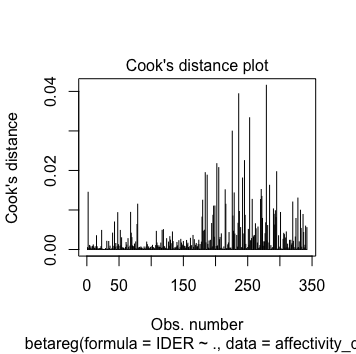
\includegraphics{assumption_plots/cook.png}
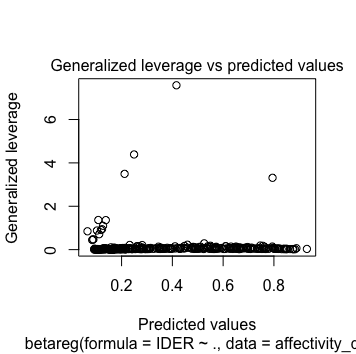
\includegraphics{assumption_plots/leverage.png}
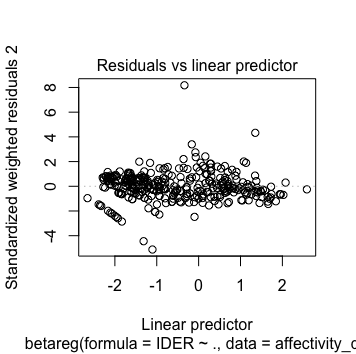
\includegraphics{assumption_plots/linear.png}
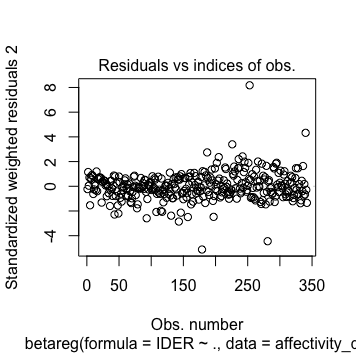
\includegraphics{assumption_plots/Residuals_observations.png}

\begin{Shaded}
\begin{Highlighting}[]
\FunctionTok{vif}\NormalTok{(beta\_fit)}
\end{Highlighting}
\end{Shaded}

\begin{verbatim}
                          Age `Disconnection and Rejection` 
                     1.235624                      4.927414 
          `Impaired Autonomy`             `Impaired Limits` 
                     3.985481                      2.564155 
         `Other-Directedness`   `Over-Vigilance/Inhibition` 
                     2.426282                      1.957390 
 `Number of Stressful Events`                           Sex 
                     1.269538                      1.094951 
       `Negative Attribution`      `Unexpected Attribution` 
                     1.722457                      1.412952 
 `Out of Control Attribution`         `Childhood Adversity` 
                     1.275194                      1.117944 
         `Physical Excercise`          `Smoking Cigarettes` 
                     1.101797                      1.194950 
                `Alcohol Use`  `Psychoactive Substance Use` 
                     1.200714                      1.188520 
\end{verbatim}

\begin{Shaded}
\begin{Highlighting}[]
\FunctionTok{tab\_model}\NormalTok{(beta\_fit,}
          \AttributeTok{title =} \StringTok{"Table 3 Beta Regression for the IDER Score in a Sample of}
\StringTok{          342 Depressed and Non{-}depressed Adults"}\NormalTok{)}
\end{Highlighting}
\end{Shaded}

\begin{longtable}[]{@{}
  >{\centering\arraybackslash}p{(\columnwidth - 6\tabcolsep) * \real{0.2500}}
  >{\centering\arraybackslash}p{(\columnwidth - 6\tabcolsep) * \real{0.2500}}
  >{\centering\arraybackslash}p{(\columnwidth - 6\tabcolsep) * \real{0.2500}}
  >{\centering\arraybackslash}p{(\columnwidth - 6\tabcolsep) * \real{0.2500}}@{}}
\caption{Table 3 Beta Regression for the IDER Score in a Sample of 342
Depressed and Non-depressed Adults}\tabularnewline
\toprule\noalign{}
\endfirsthead
\endhead
\bottomrule\noalign{}
\endlastfoot
~ &
\multicolumn{3}{>{\centering\arraybackslash}p{(\columnwidth - 6\tabcolsep) * \real{0.7500} + 4\tabcolsep}@{}}{%
IDER} \\
Predictors & Estimates & CI & p \\
(Intercept) & 0.16 & 0.07~--~0.35 & \textbf{\textless0.001} \\
Age & 0.99 & 0.98~--~1.00 & \textbf{0.011} \\
\begin{minipage}[t]{\linewidth}\raggedright
Disconnection and\\
Rejection\strut
\end{minipage} & 1.07 & 1.03~--~1.10 & \textbf{\textless0.001} \\
Impaired Autonomy & 1.08 & 1.05~--~1.12 & \textbf{\textless0.001} \\
Impaired Limits & 1.02 & 0.99~--~1.04 & 0.126 \\
Other-Directedness & 1.00 & 0.98~--~1.03 & 0.939 \\
Over-Vigilance/Inhibition & 1.00 & 0.98~--~1.03 & 0.962 \\
\begin{minipage}[t]{\linewidth}\raggedright
Number of Stressful\\
Events\strut
\end{minipage} & 1.00 & 0.99~--~1.01 & 0.785 \\
Sex {[}Male{]} & 1.07 & 0.88~--~1.31 & 0.477 \\
Negative Attribution {[}No{]} & 0.66 & 0.53~--~0.83 &
\textbf{\textless0.001} \\
\begin{minipage}[t]{\linewidth}\raggedright
Unexpected Attribution\\
{[}No{]}\strut
\end{minipage} & 1.04 & 0.85~--~1.28 & 0.675 \\
\begin{minipage}[t]{\linewidth}\raggedright
Out of Control\\
Attribution {[}No{]}\strut
\end{minipage} & 0.74 & 0.59~--~0.94 & \textbf{0.012} \\
Childhood Adversity {[}No{]} & 0.71 & 0.59~--~0.86 &
\textbf{\textless0.001} \\
Physical Excercise {[}No{]} & 1.03 & 0.86~--~1.23 & 0.773 \\
Smoking Cigarettes {[}No{]} & 0.75 & 0.60~--~0.95 & \textbf{0.015} \\
Alcohol Use {[}No{]} & 0.95 & 0.74~--~1.23 & 0.707 \\
\begin{minipage}[t]{\linewidth}\raggedright
Psychoactive Substance\\
Use {[}No{]}\strut
\end{minipage} & 1.43 & 0.86~--~2.38 & 0.165 \\
Observations &
\multicolumn{3}{>{\raggedright\arraybackslash}p{(\columnwidth - 6\tabcolsep) * \real{0.7500} + 4\tabcolsep}@{}}{%
342} \\
R\textsuperscript{2} &
\multicolumn{3}{>{\raggedright\arraybackslash}p{(\columnwidth - 6\tabcolsep) * \real{0.7500} + 4\tabcolsep}@{}}{%
0.596} \\
\end{longtable}




\end{document}
